\section{APÊNDICE V - LEGENDAS À REPRESENTAÇÃO ESPACIAL DOS AGENTES}

A Figura \ref{fig:legendaAgentesHumanos} apresenta o significado dos ícones utilizados na representação dos agentes humanos. Cada formato geométrico distinto indica uma faixa etária e as cores indicam o estado do agente de acordo com o modelo. Considera-se interessante categorizar as representações gráficas de acordo com a população para que seja possível realizar o acompanhamento dos agentes durante o período de tempo considerado pelas simulações executadas.

\begin{figure}[H]
  \centering
  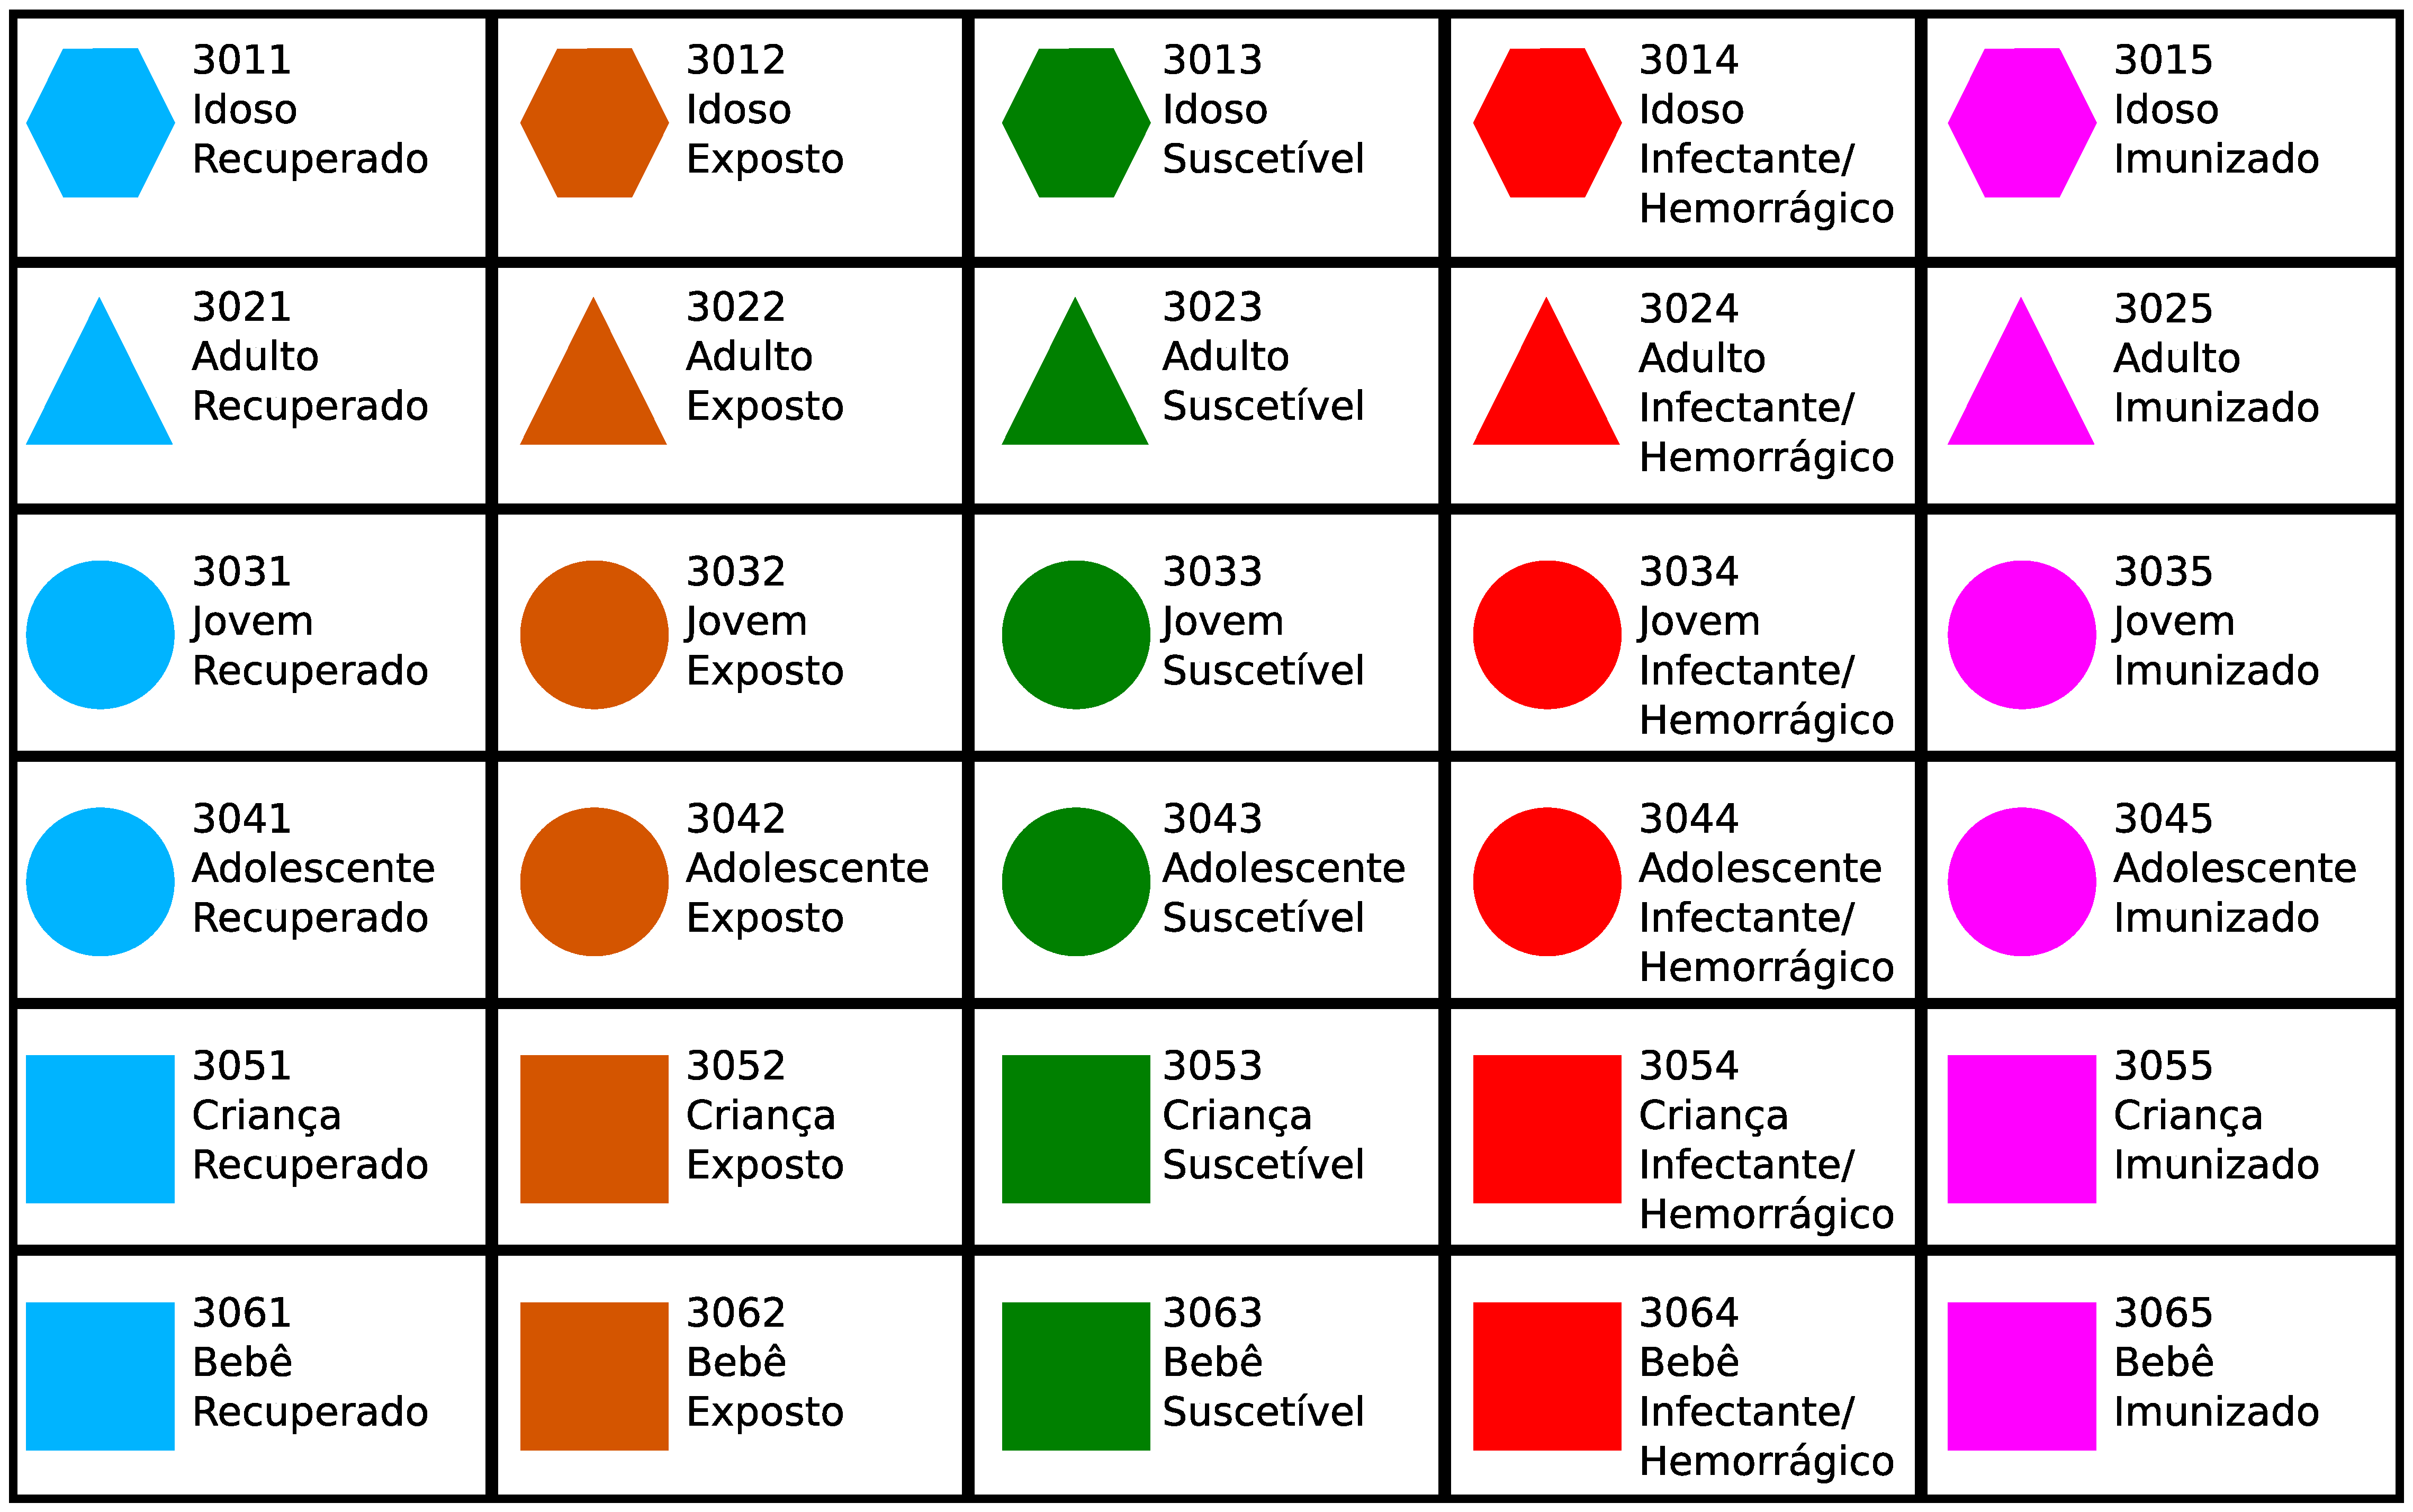
\includegraphics[width=0.8\textwidth]{Figuras/A5/AgentesHumanos.eps}
  \caption{Legenda dos ícones utilizados à representação dos distintos tipos de agentes humanos.}
  \label{fig:legendaAgentesHumanos}
\end{figure} 

\newpage
